\documentclass[mode=present, paper=screen, display=slides, style=horatio,
hlsections=true]{powerdot}
% Buradaki paper boyu önemli.
% smartboard yapınca ciddi anlamda büyük bir alan tanımlanıyor.
% a4paper, letterpaper seçenekleri var.
% screen 4/3 oranında bildiğimiz ekran.
\usepackage[utf8]{inputenc}
\usepackage[overlay]{textpos}
\setlength{\TPHorizModule}{10mm}
\setlength{\TPVertModule}{10mm}
\usepackage{pgfplots}
\pgfplotsset{compat=1.12, height=0.45\slideheight}
\usepackage{amsfonts}
\usepackage{pgfplots}
\pgfplotsset{width=7cm,compat=1.12}
\DeclareMathAlphabet{\mathpzc}{OT1}{pzc}{m}{it}

% Buradaki mavi gerçek İTÜ mavisi değil ama logonun arka planı böyle verilmiş. Ben de
% ona uyuyorum.
\pddefinepalettes{itu}{
\definecolor{pdcolor1}{RGB}{16,64,118}
\definecolor{pdcolor2}{RGB}{139,115,74}
\pddefinetemplate[slide]{slide}{lffont=\footnotesize\color{white}}{}
\pddefinetemplate[slide]{slide}{cffont=\footnotesize\color{white}}{}
\pddefinetemplate[slide]{slide}{rffont=\footnotesize\color{white}}{}
\pddefinetemplate[titleslide]{titleslide}{lffont=\footnotesize\color{white}}{}
\pddefinetemplate[titleslide]{titleslide}{cffont=\footnotesize\color{white}}{}
\pddefinetemplate[titleslide]{titleslide}{rffont=\footnotesize\color{white}}{}
\pddefinetemplate[slide]{slide}{tocfont=\scriptsize\raggedright}{}
}

\pdsetup{
palette=itu,
logohook=t,
logopos={0.0815\slidewidth,0.987\slideheight},
logocmd={
\includegraphics[height=0.12\slideheight]{itulogo.eps}},
lf=,
cf=,
rf=,
% Bunlar rasgele yuvarlaklar çıkaran komutlar, pek gerekli değil.
% randomdots,
% dmindots=25,
% dmaxdots=35,
% dminsize=6pt,
% dmaxsize=25pt,
% dminwidth=.82\slidewidth,
% dmaxwidth=.97\slidewidth,
% dminheight=.88\slideheight,
% dmaxheight=.96\slideheight,
% dbright=60,
}

% Bunlar gerekli olabilecek fazladan ortamları tanımlamak için.
\newenvironment{description1}%
  {\begin{list}{}{\setlength{\labelwidth}{0pt}
   \setlength{\itemindent}{-18pt}
   \renewcommand{\makelabel}{\descriptionlabel}}}%
  {\end{list}}

\newenvironment{description2}%
  {\begin{list}{}{\setlength{\labelwidth}{0pt}
   \setlength{\itemindent}{-\leftmargin}
   \renewcommand{\makelabel}{\descriptionlabel}}}%
  {\end{list}}

\newenvironment{description3}%
  {\begin{list}{}{\setlength{\labelwidth}{0pt}
   \setlength{\itemindent}{-36pt}
   \renewcommand{\makelabel}{\descriptionlabel}}}%
  {\end{list}}


\title{Developing An Ontology for GIS-based Decision Support System to Determine River Pollution}
\author{Recep Can Altınbağ\\150130065\\ \\Advisor: Asst. Prof. Dr. Mehmet Tahir SANDIKKAYA}
\date{2018\ \\\
\\Istanbul Technical University\\Faculty of Computer And Informatics}

\begin{document}
 
\maketitle

\begin{slide}[toc=,bm=]{Overview}
\vspace{2em}\footnotesize\tableofcontents[content=all]
\end{slide}

%%%%%%%%%%%%%%%%%%%%%%%%%%%%%%%
%%%%%     1. BÖLÜM
%%%%%%%%%%%%%%%%%%%%%%%%%%%%%%%
\section{Problem Definition}

%toc içine yazılan "içerik" içinde görülür.
\begin{slide}{Problem Definition}
  \begin{itemize}
    \item Representation of data 
    \begin{itemize}
    	\pause\item Geographical Information Systems
        
        \begin{figure}[H]
    \centering
    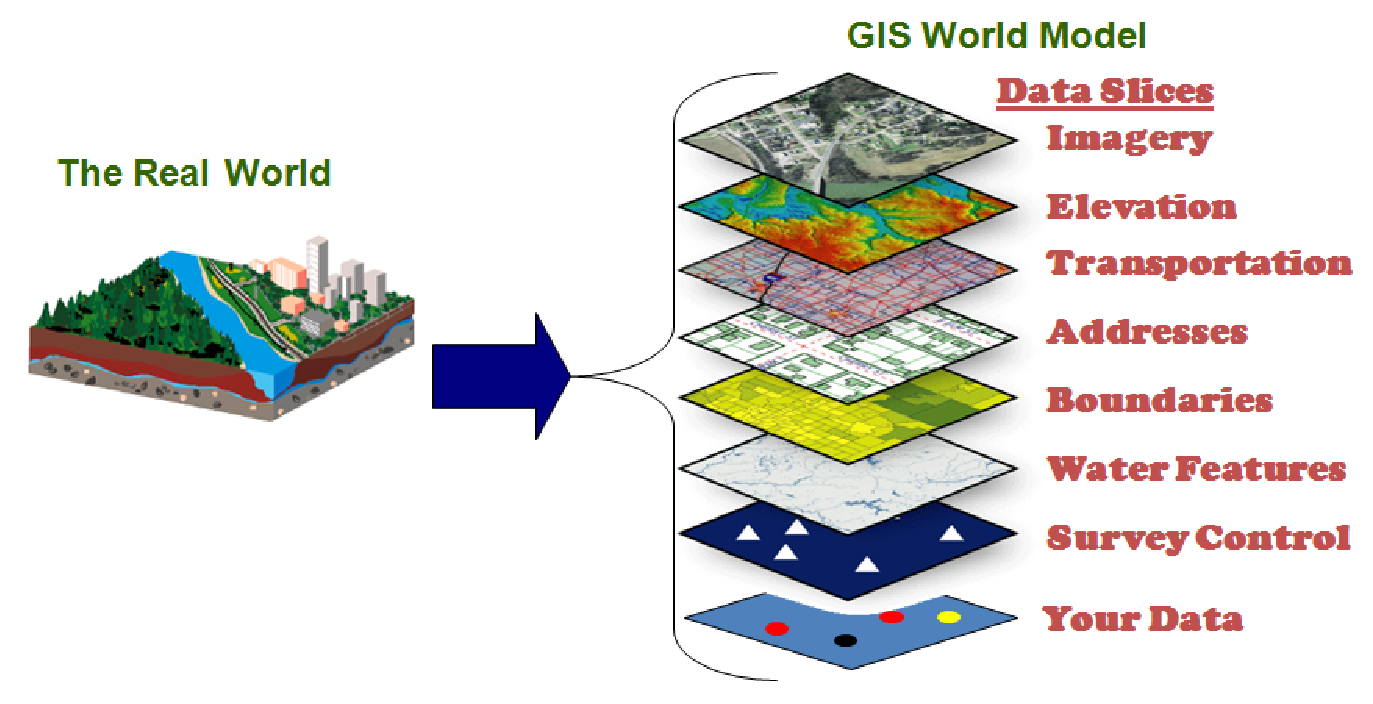
\includegraphics[width=.6\linewidth]{3.eps}
    \caption{Reference: https://henrico.us/it/gis/}
    \label{fig:prefix4}
\end{figure}
        
        
		\pause\item Semantic Web 
    \end{itemize}
  \end{itemize}




\end{slide}

\begin{slide}[toc=Semantic Web]{Semantic Web}
  
 

\begin{figure}[H]
    \centering
    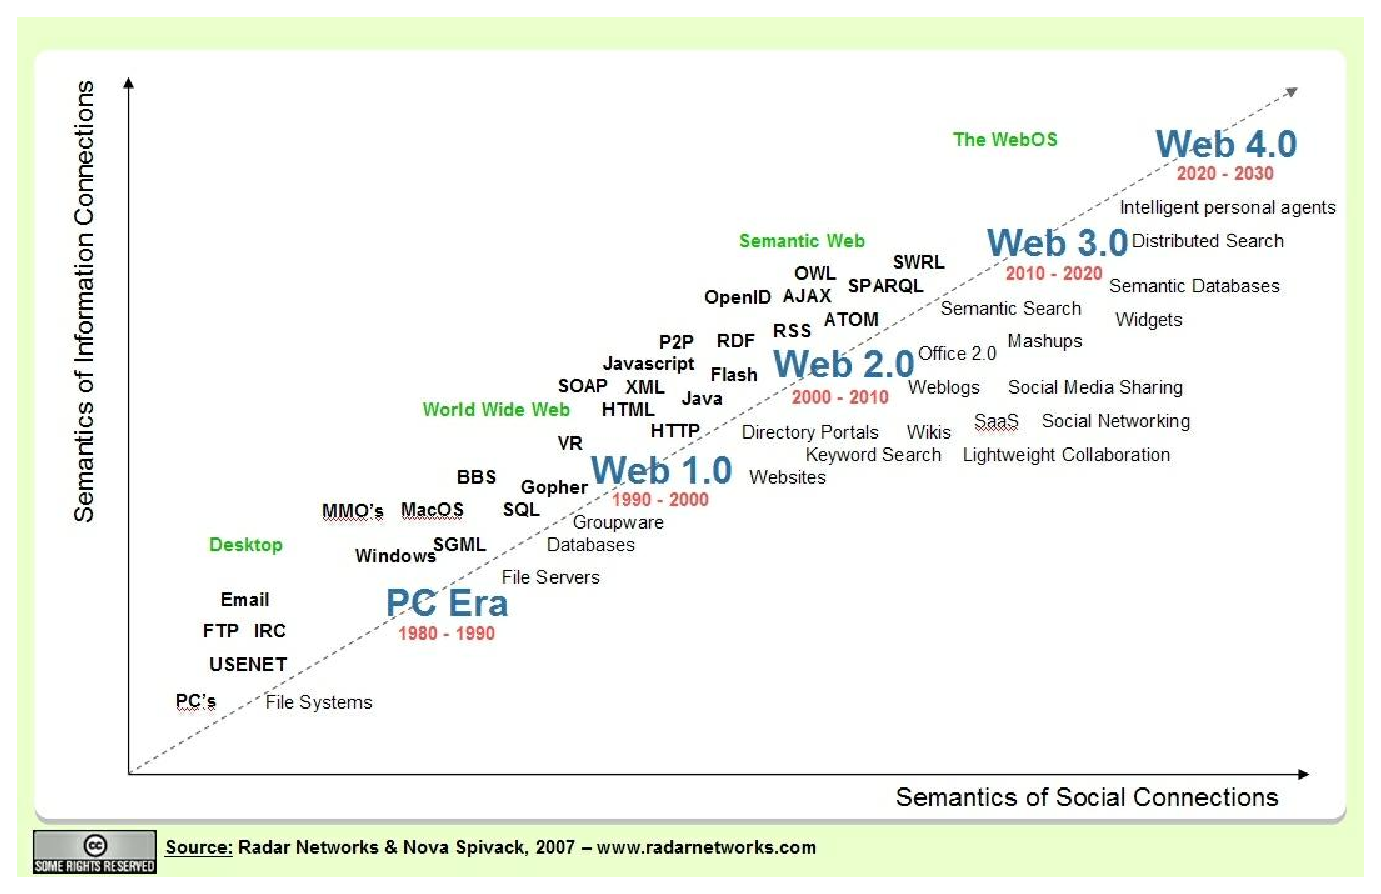
\includegraphics[width=.8\linewidth]{4.eps}
    \caption{Reference: https://www.w3.org/RDF/Metalog/docs/sw-easy}
    \label{fig:prefix3}
\end{figure}
  
    



\end{slide}

%%%%%%%%%%%%%%%%%%%%%%%%%%%%%%%
%%%%%     2. BÖLÜM
%%%%%%%%%%%%%%%%%%%%%%%%%%%%%%%
\section{Ontology Development}

\begin{slide}[toc=Semantic Web Layers]{Semantic Web Layers}
  
  \begin{figure}[H]
    \centering
    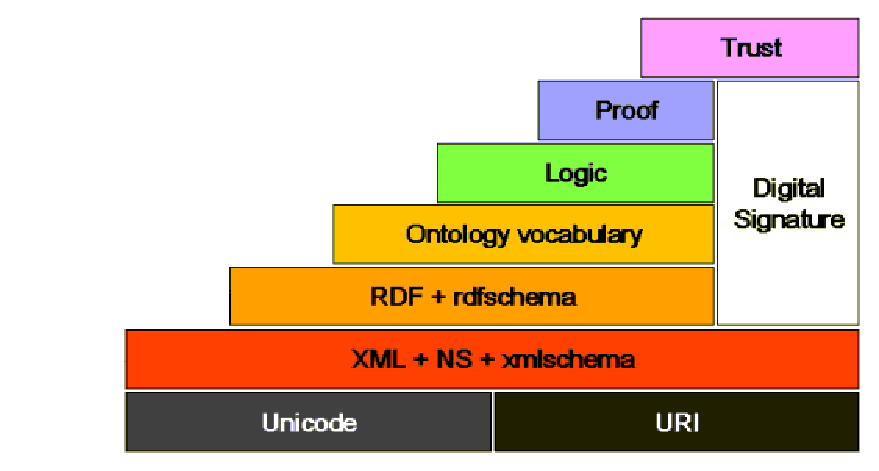
\includegraphics[width=.6\linewidth]{6.eps}
    \caption{Reference: https://www.w3.org/RDF/Metalog/docs/sw-easy}
    \label{fig:prefix1}
\end{figure}

URI,URL: Source of data.
XML: structural files
RDF: data model, object(source)-relation(source)-subject(source) \\
OWL: More Complex Vocabulary, Rules, Inference, Knowledge Extraction, Reasoning



  

\end{slide}

\begin{slide}[toc=Ontology Development]{Ontology Development Process}
  
 \begin{figure}[H]
    \centering
    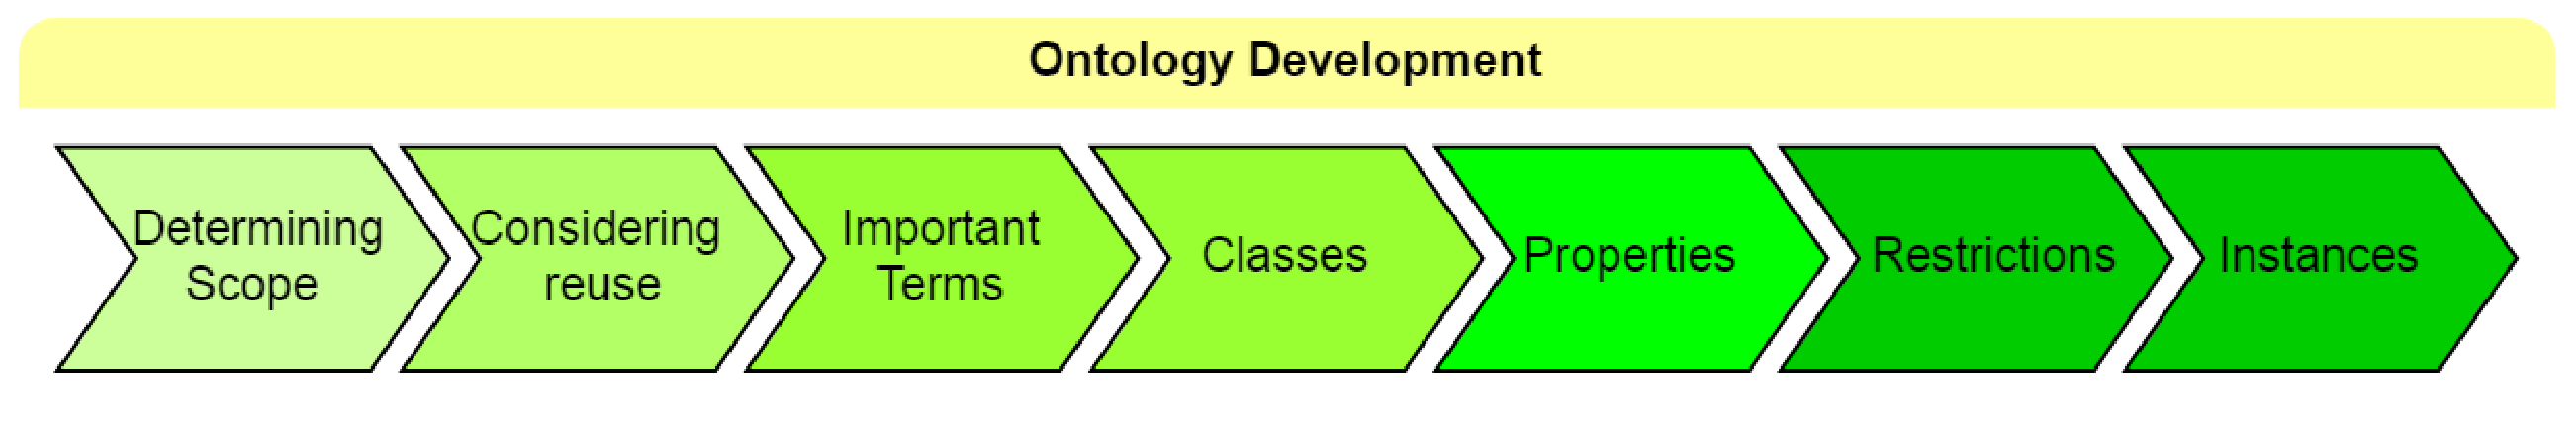
\includegraphics[width=.9\linewidth]{10.eps}
    \label{fig:prefix5}
\end{figure}
\begin{itemize}
    	\pause\item Water Management Project which consist of relations between observations, measurements, pollutants, sources, rivers, units
        \pause\item different requirements and scopes
        \pause\item Industry, Measurement of Quantity, Spatial, Pollutants, Pollution Sources
        \pause\item Object and Data Properties
        \pause\item Role Restrictions of Properties
        \pause\item Units, Prefixes, Pollutants, Pollutant Features
\end{itemize}



\end{slide}

\section{Ontology Model with Use Cases}

\begin{slide}[toc=Measurement]{An Example of Measurement}
  
    
 \begin{figure}[H]
    \centering
    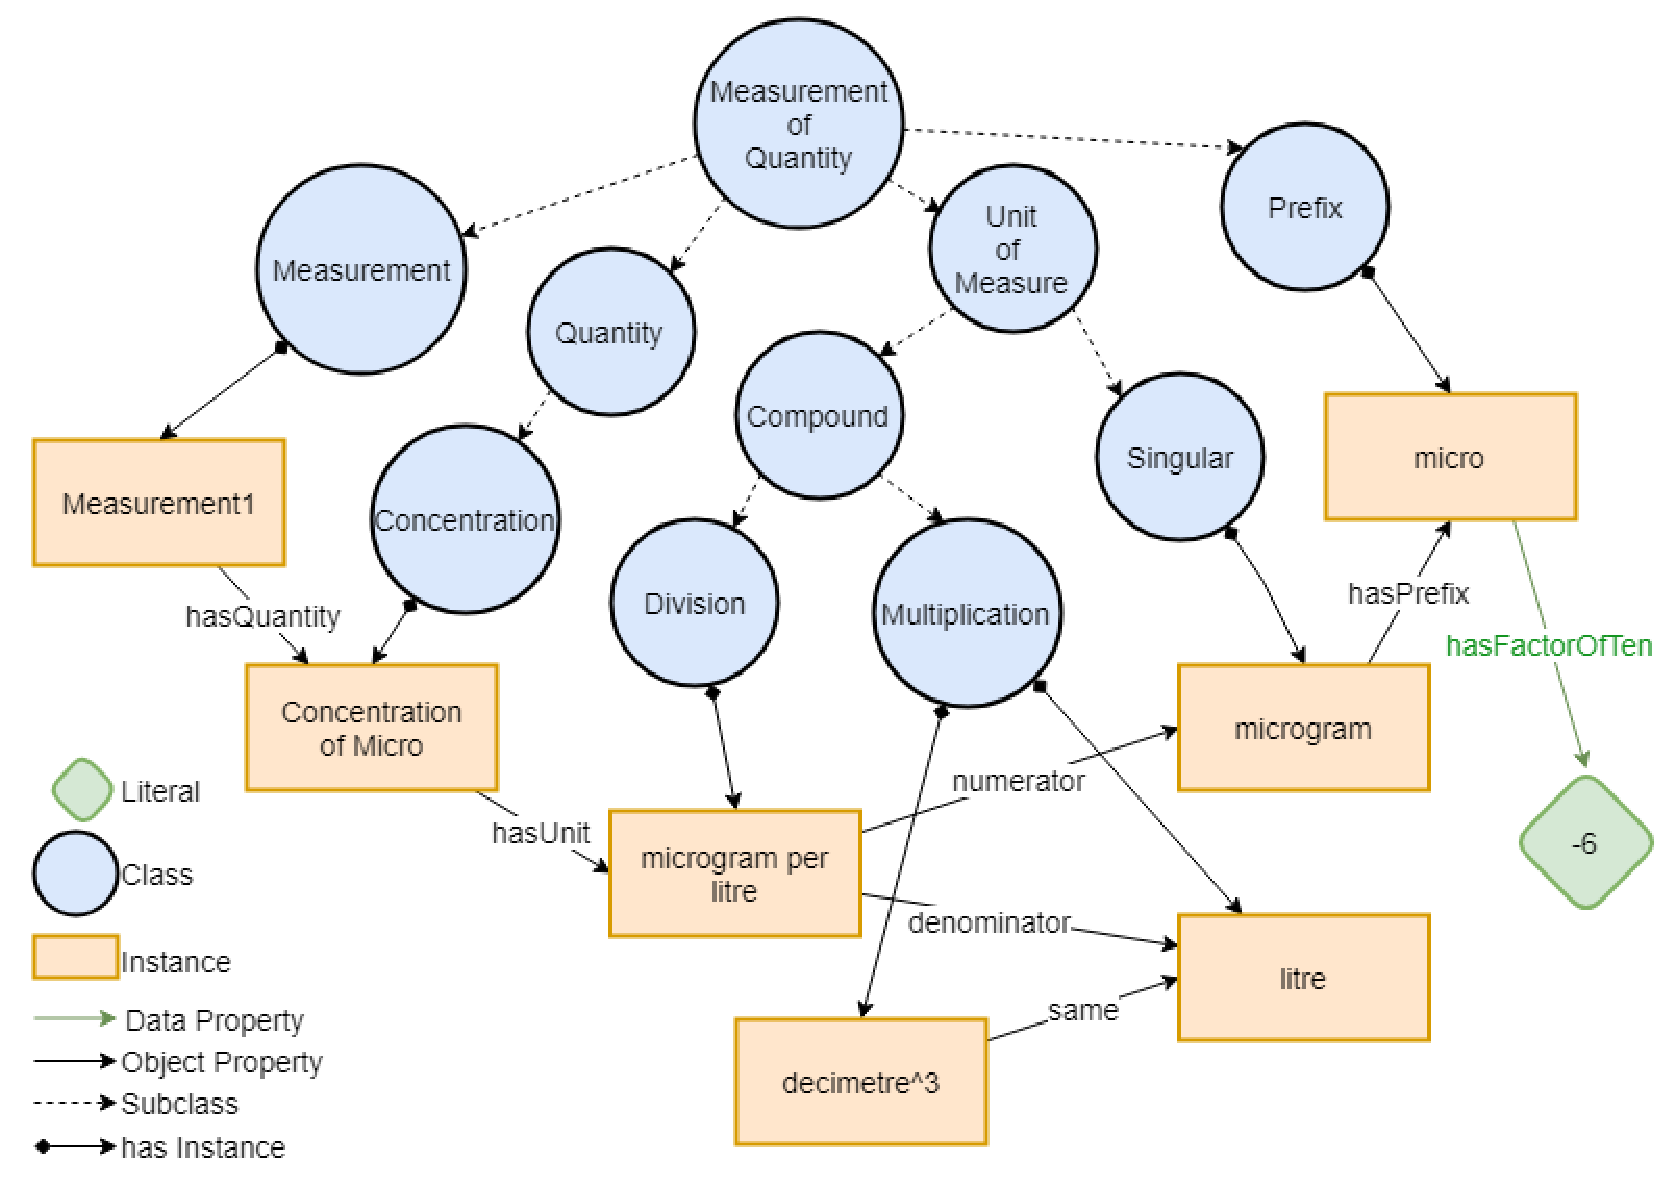
\includegraphics[width=.9\linewidth]{11.eps}
    \label{fig:prefix6}
\end{figure}
  
 

\end{slide}

\begin{slide}[toc=Pollutant]{An Example of Pollutant and Features}
      
 \begin{figure}[H]
    \centering
    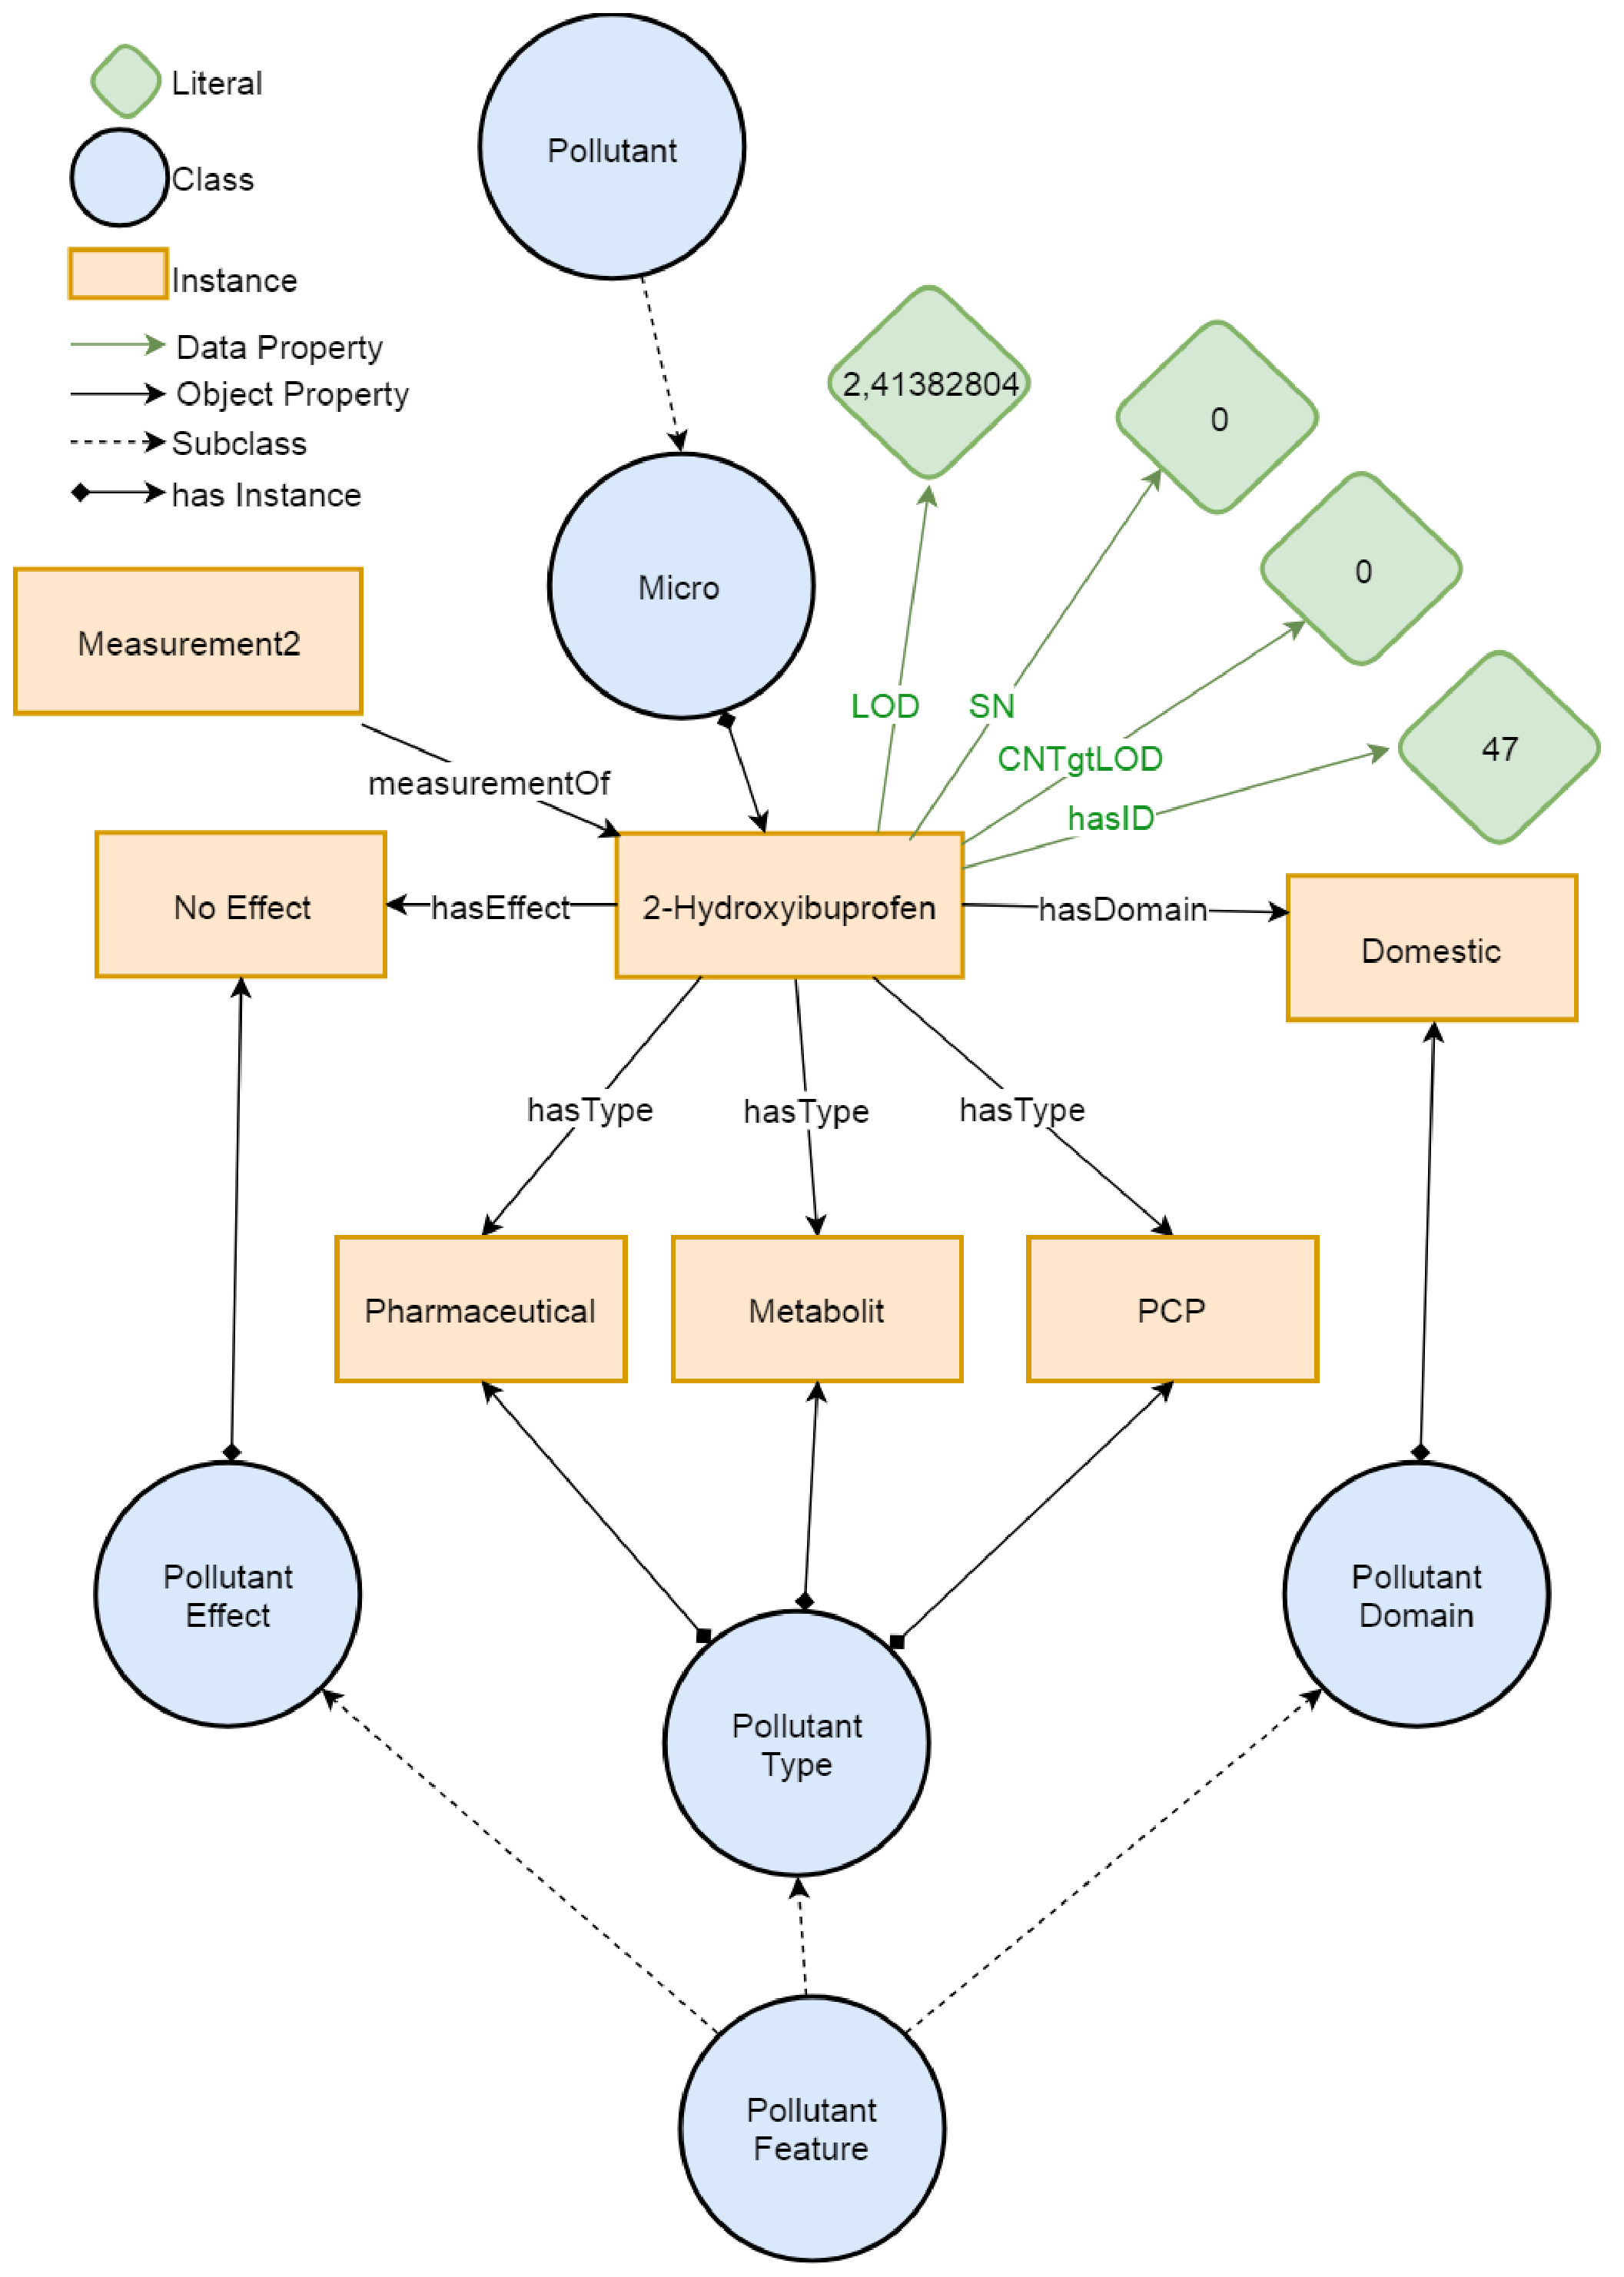
\includegraphics[width=.48\linewidth]{12.eps}
    \label{fig:prefix8}
\end{figure}
\end{slide}

\begin{slide}[toc=Observer]{Observer Relations}
      
 \begin{figure}[H]
    \centering
    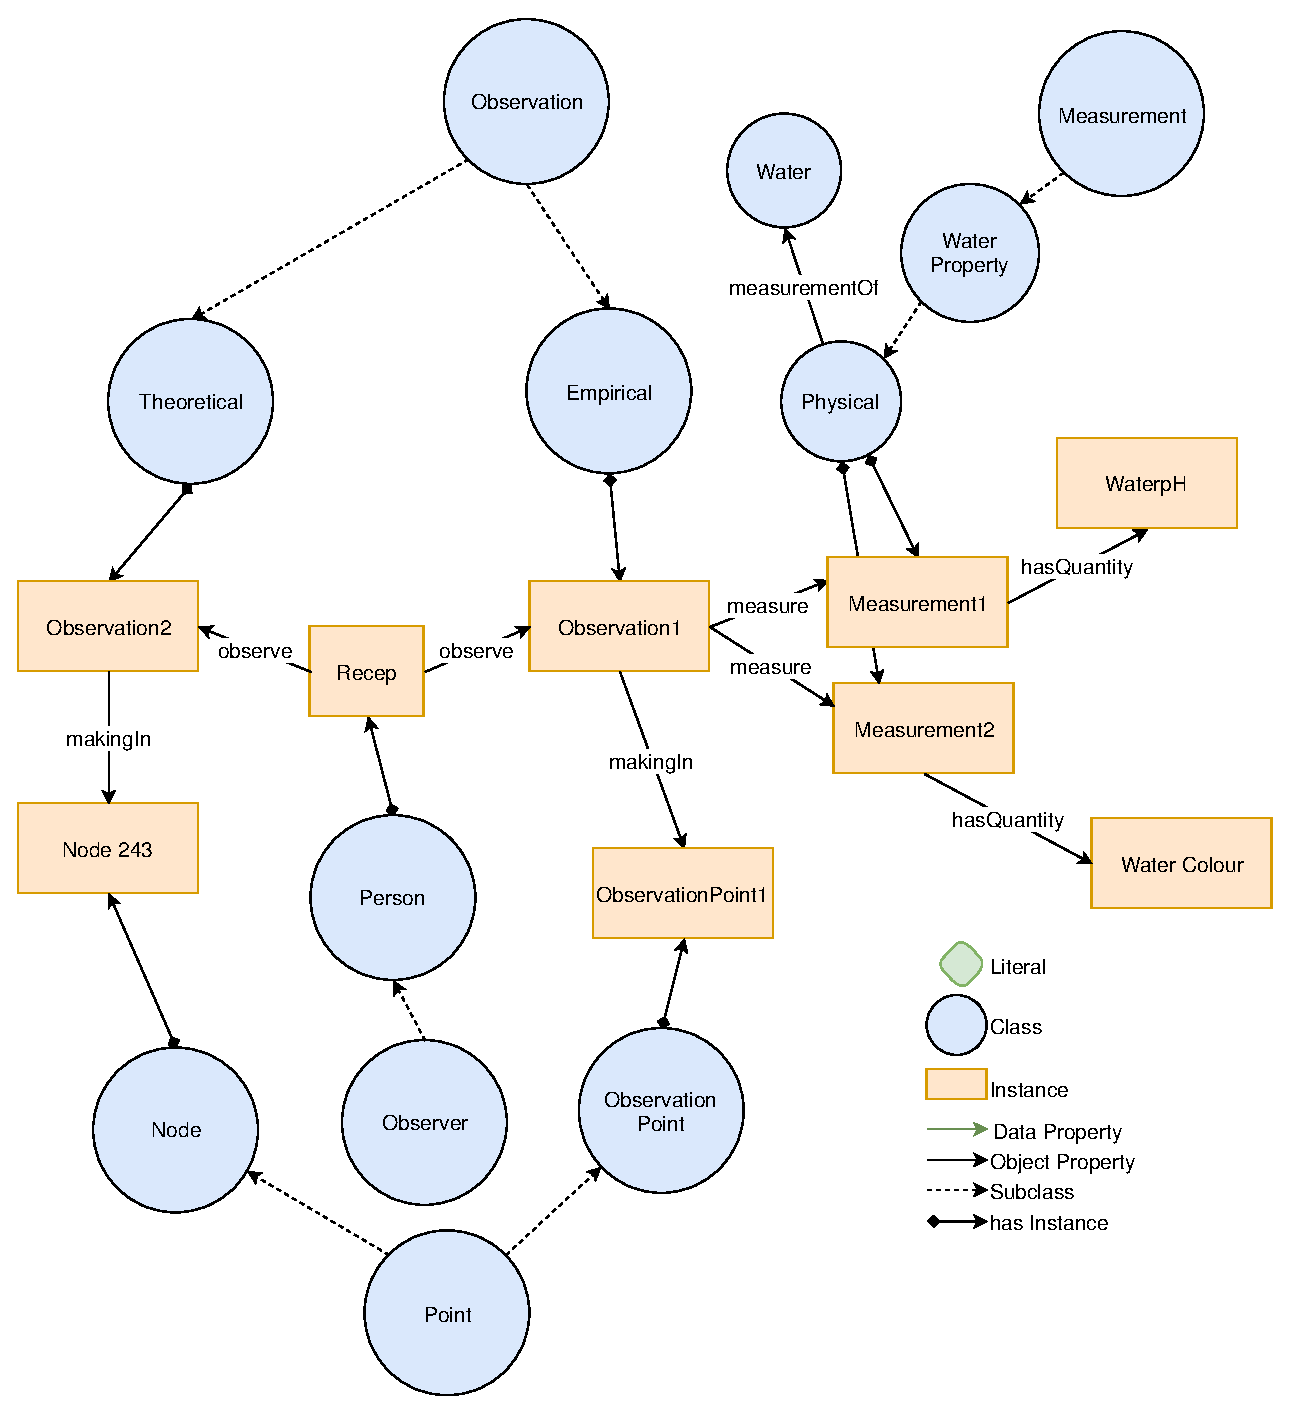
\includegraphics[width=.58\linewidth]{15.eps}
    \label{fig:prefix7}
\end{figure}
\end{slide}

\begin{slide}[toc=River]{River Representation}
      
 \begin{figure}[H]
    \centering
    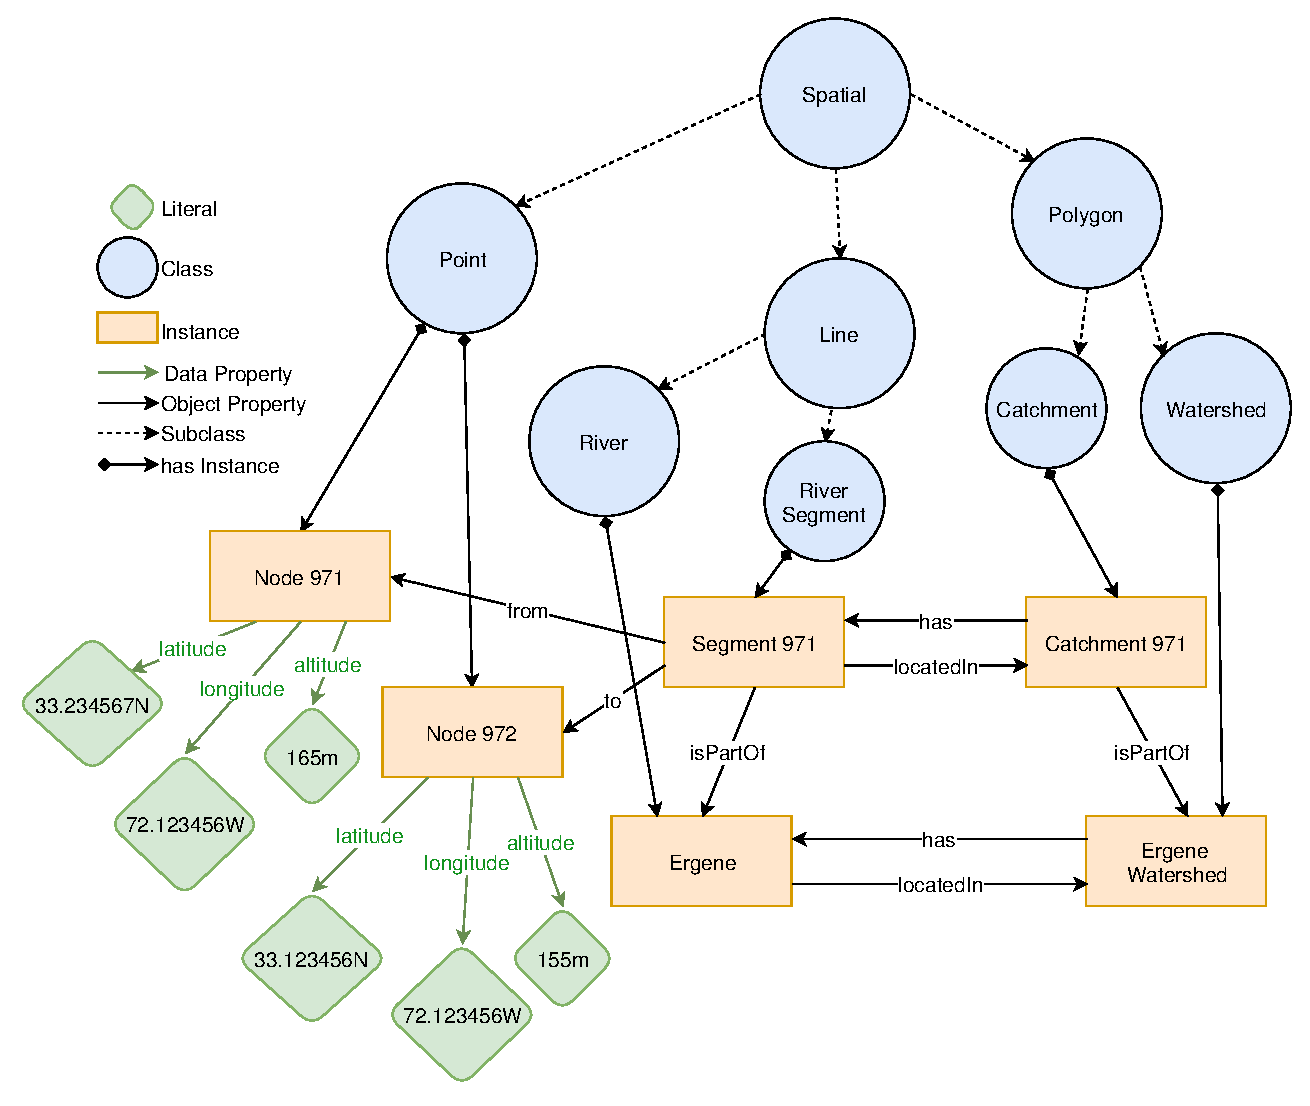
\includegraphics[width=.68\linewidth]{16.eps}
    \label{fig:prefix9}
\end{figure}
\end{slide}

\begin{slide}[toc=Pollution Sources]{Pollution Sources}
      
 \begin{figure}[H]
    \centering
    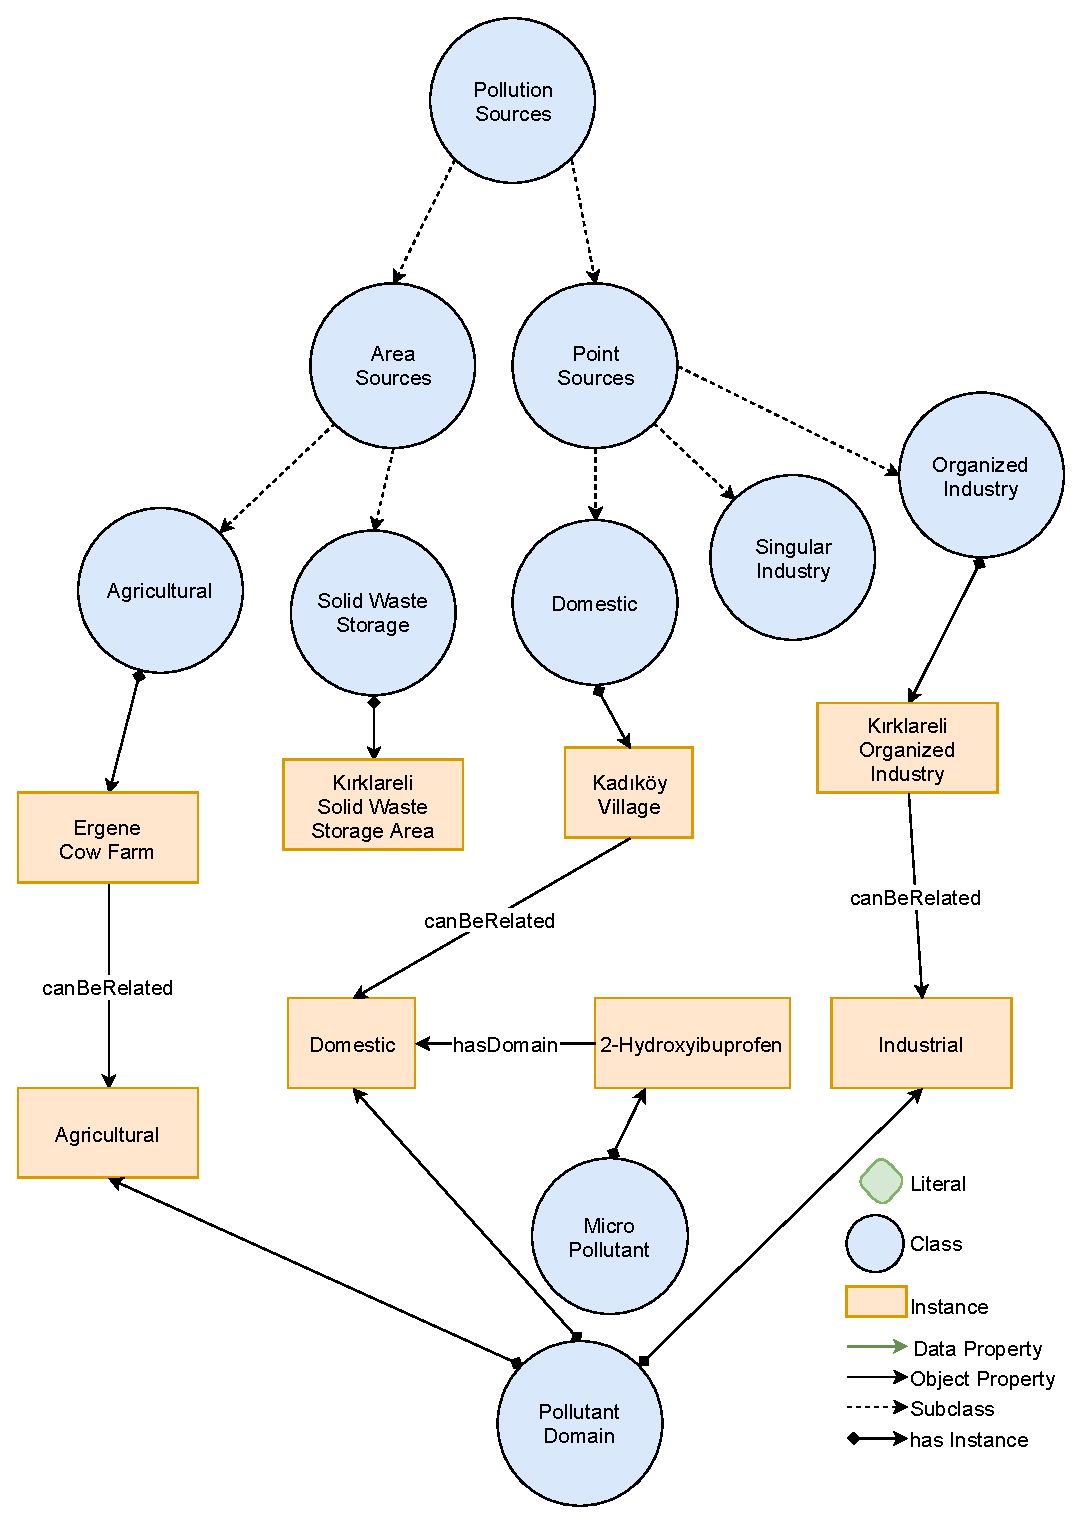
\includegraphics[width=.43\linewidth]{17.eps}
    \label{fig:prefix11}
\end{figure}
\end{slide}



\section{Reasoning and Querying}

\begin{slide}[toc=Reasoning and Querying]{Reasoning and Querying}
  
  
  \begin{itemize}
    \item  2834
axioms, 71 classes, 25 object properties, 20 data properties, 4 annotation properties
and 437 individual
    \pause\item reasoner helps to find contradictions among axioms and semantic querying
  \end{itemize}
  \begin{figure}[H]
    \centering
    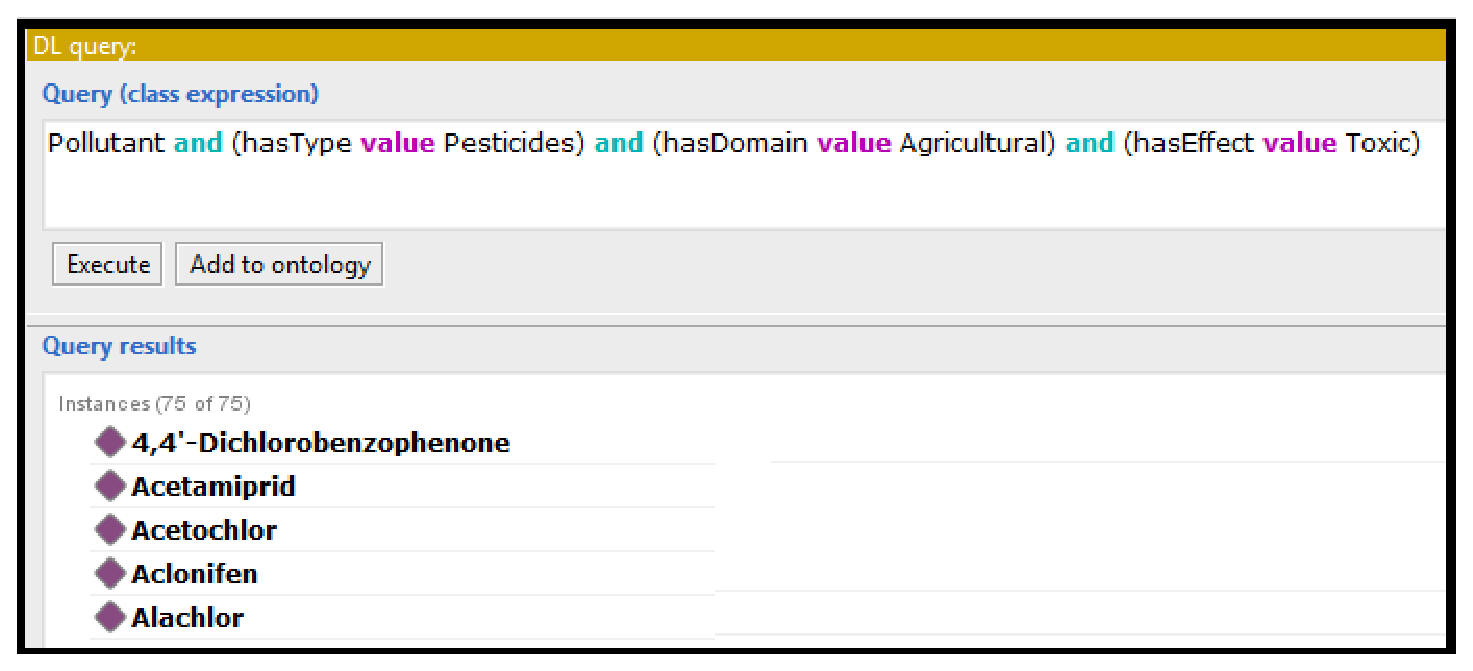
\includegraphics[width=.9\linewidth]{13.eps}
    \label{fig:prefix12}
\end{figure}

\end{slide}

\section{Conclusion and Future Work}

\begin{slide}[toc=Conclusion]{Conclusion}
  \begin{itemize}
    \item Semantic Web approach was used 
    \pause\item For water
management projects 
	\pause\item Concepts and relations in the real life objects were divided into parts, use cases were used 
    \pause\item Querying with DLQuery and owlready2 are used to extract more
information and automate of the evaluating process  
  \end{itemize}
  \begin{figure}[H]
    \centering
    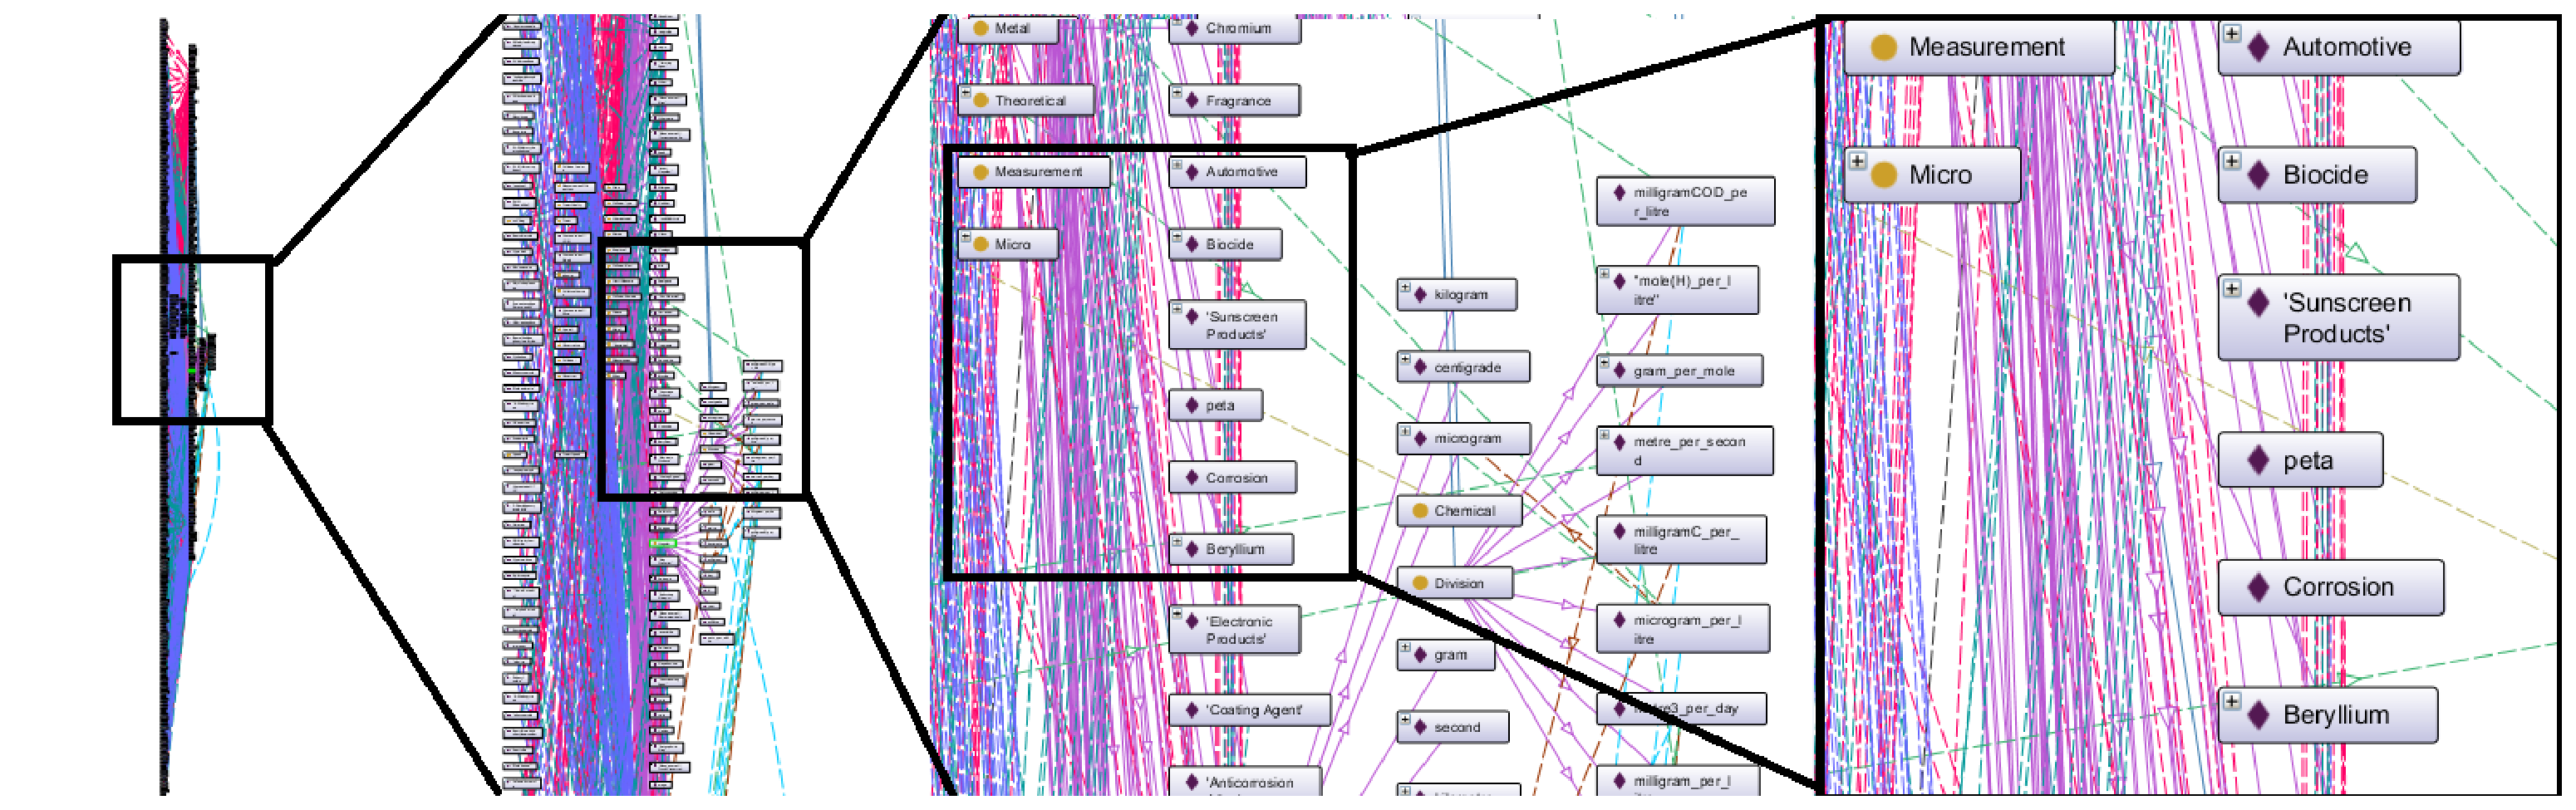
\includegraphics[width=.9\linewidth]{14.eps}
    \label{fig:prefix13}
\end{figure}

\end{slide}


\begin{slide}[toc=Final Version]{Final Version}
\begin{figure}[H]
    \centering
    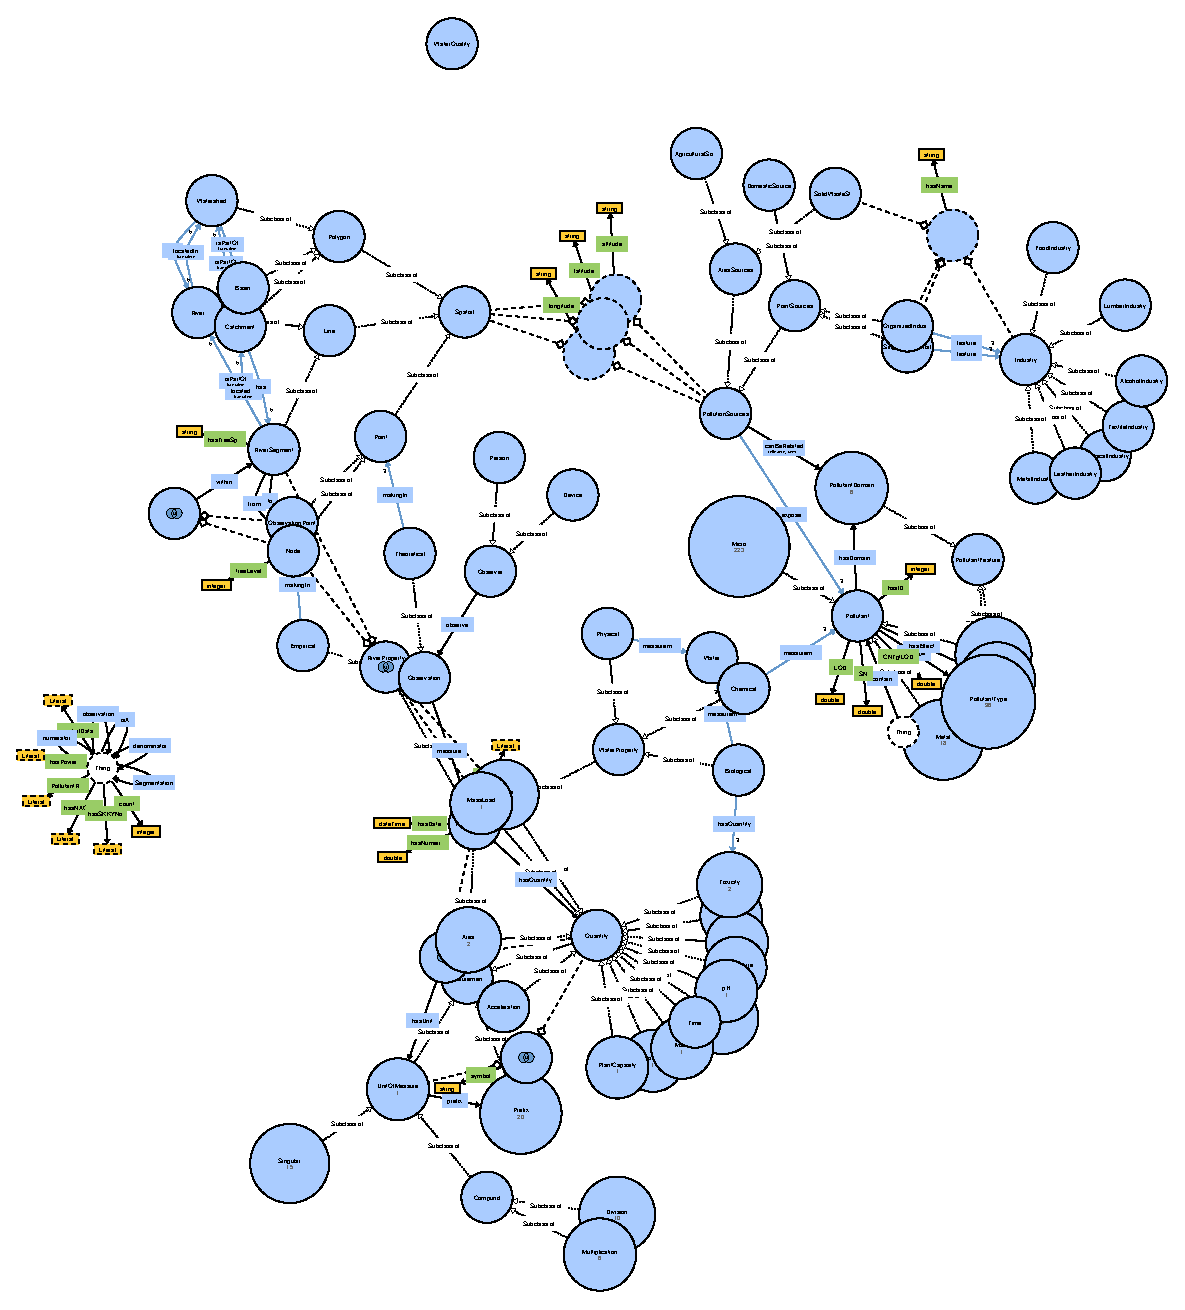
\includegraphics[width=.6\linewidth]{2.eps}
    \label{fig:prefix14}
\end{figure}
\end{slide}

\begin{slide}[toc=Future Work]{Future Work}
  \begin{itemize}
    \item Converting data to RDF type
    \pause\item Connecting autonomous data collecting device with the ontology knowledge domain  
	\pause\item Going up though Semantic Web layers
    
  \end{itemize}
 

\end{slide}


\begin{slide}[toc=Demo]{Demo}

\end{slide}

\begin{slide}[]{}
Thank you for listening
\end{slide}



\end{document}